\section{Gluing the finite groups without collapsing them}\label{sec:gluing}

The quotient $G_0$ of Section~\ref{op:modular-section} identifies a cyclic
subgroup across each edge of $\Gamma$. It must
retain every vertex group: otherwise a later nonzero element of a finite
group algebra could disappear.  We first prove a general injectivity
criterion and then verify it for the groups used here.  The local
injectivity argument belongs to the $C(4)$--$T(4)$ theory of graphical
complexes of groups \cite[Section~8]{Prytula2024}.  We give a direct
proof using only labelled spherical maps and Euler's formula.

\subsection{An injectivity criterion}

\begin{lemma}[Triangle-free gluing]\label{lem:triangle-free-gluing}
Let $\Delta$ be a finite simple triangle-free graph.  For each vertex $i$,
let $D_i$ be a finite group.  For each edge $\gamma=\{i,j\}$, let
$C_\gamma$ be a nontrivial finite cyclic group, with injective homomorphisms
$\iota_{\gamma,i}:C_\gamma\to D_i$ and
$\iota_{\gamma,j}:C_\gamma\to D_j$.
Assume the following condition at every vertex $i$.  If $1\leq k\leq3$,
the edges $\gamma_1,\ldots,\gamma_k$ are incident to $i$, and
$s_a\in C_{\gamma_a}\setminus\{1\}$, then
\begin{equation}\label{eq:gluing-short-word}
 \iota_{\gamma_1,i}(s_1)\cdots
 \iota_{\gamma_k,i}(s_k)\neq1
\end{equation}
whenever consecutive edge labels are distinct cyclically.  For $k=1$
the distinctness condition is omitted; for $k\geq2$ it includes
$\gamma_k\neq\gamma_1$.
Then every natural homomorphism $D_i\to Q$ is injective, where
\[
 Q=\left(*_{i\in V(\Delta)}D_i\right)
 \big/\left\langle\!\left\langle
 \iota_{\gamma,i}(s)\iota_{\gamma,j}(s)^{-1}:
 \gamma=\{i,j\},\ s\in C_\gamma
 \right\rangle\!\right\rangle.
\]
\end{lemma}

\begin{proof}
We first handle the subgroups generated by the incident cyclic groups.
The diagram argument will rule out a relation that is nontrivial at one
vertex but follows from the relations at all the vertices.  At the end,
a permutation action extends the conclusion to the full groups $D_i$.

Put
\[
 D_i^0=\langle\iota_{\gamma,i}(C_\gamma):\gamma\ni i\rangle.
\]
Choose a generator of each $C_\gamma$, and let $L$ have one generator
$x_\gamma$ for each edge.  Its defining relators are all words in the
$x_\gamma^{\pm1}$ incident to a single vertex that evaluate to $1$ in
that vertex group.  There is a well-defined map $D_i^0\to L$: two words
representing the same element of $D_i^0$ differ by one of these relators.

\paragraph{A failed injection produces a spherical map.}
Suppose a nonidentity element of $D_i^0$ maps to $1$ in $L$, and choose a
word $w$ representing it.  There is a finite sequence of words from $w$
to the empty word, each step inserting or deleting a defining relator,
its inverse, or a free inverse pair.  Indeed, membership in the normal
closure of the relators expresses $w$ in the free group as a finite
product of conjugates of relators; free insertions and cancellations
reach such a product, and the conjugated relators can then be erased.

We describe the spherical maps needed to encode this sequence.  A map
is a finite connected graph drawn tamely on the sphere, allowing loops
and parallel edges.  An edge is either \emph{neutral}, with value $1$,
or is labelled by an edge $\gamma$ of $\Delta$.  In the latter case its
two oriented traversals, called darts, have mutually inverse values in
$C_\gamma\setminus\{1\}$.  Every face has a type $i\in V(\Delta)$
incident to every label in its boundary walk.  Its boundary word is
evaluated in $D_i$, using the specified embeddings. A face is
\emph{ordinary} when this evaluation is the identity. Call the map
\emph{exceptional} if precisely one face has nonidentity evaluation and
all other faces have identity evaluation.  Changing the starting point
conjugates a boundary product, and reversing the walk inverts it, so
identity versus nonidentity is well-defined.

Draw the successive words in horizontal levels of a rectangle, with
each letter an oriented edge.  Represent an empty level by a single
neutral edge.  In every intervening strip join corresponding vertices
along the unchanged prefix and suffix by noncrossing neutral edges.
At an insertion or deletion, join the single insertion vertex on the
shorter path to the two endpoints of the inserted block on the longer
path.  The strip faces then read either a letter followed by its inverse,
or the inserted relator, with neutral edges interspersed.  If a level is
empty, the adjacent nonempty word is the entire inserted or deleted
block; one face between these two levels suffices.  Assign the relator's
vertex type to its face, and either endpoint type of a letter's label
to an unchanged-letter face.  All these faces evaluate to $1$.  Include
the neutral edges along the two vertical sides of the rectangle.  The
exterior face has word $w$ or $w^{-1}$, apart from neutral edges; give it
type $i$.  This connected drawing, viewed on the sphere, is exceptional.

We shall prove that no exceptional map exists.  Choose one with the
smallest possible number of edges.  This number is positive: the only
face of an isolated vertex has the empty word, which evaluates to $1$.
The reductions below will make every vertex degree and every ordinary
face length at least four away from a possible loop. Euler's formula
will then rule out both the loop-free case and the remaining one-loop
case.

\paragraph{Boundary walks and elementary reductions.}
Fix an orientation of the sphere.  At each vertex let $\sigma$ be the
cyclic successor of outgoing darts and let $\alpha$ reverse a dart.
Boundary walks are the cycles of $\sigma\alpha$: after traversing a
dart, take the successor of its reverse.  For a disconnected drawing we
use each component's own boundary walks, counting one empty walk for
an isolated vertex.  If a drawing has $v$ vertices, $e$ edges, $F$ such
walks and $c$ components, then
\begin{equation}\label{eq:gluing-euler}
 v-e+F=2c.
\end{equation}
For completeness, in a connected spherical drawing a nonbridge edge
lies on a simple circuit.  Its two sides are therefore on distinct
boundary walks; deleting it merges those walks and preserves
connectedness.  Repeated deletion leaves a tree, which has one boundary
walk and $e=v-1$.  This proves the formula for a connected drawing;
summing proves the displayed formula.  The same walk rules follow by
taking small vertex discs and thin edge bands.

A neutral nonloop edge can be contracted, with its neutral darts
omitted from the boundary words.  This preserves every face evaluation
and contradicts minimality.  For a neutral loop based at $b$, retain
the closed side containing the exceptional face, then remove the loop.
The retained graph is connected: each side of the loop attaches to the
other only at $b$.  The other dart slots on the retained side form an
interval between the loop slots; closing that interval gives precisely
the old walks on that side with the neutral loop dart removed.  Thus
their evaluations are unchanged.  If only $b$ remains, its walk is empty
and could not be exceptional.  In every possible case a smaller
exceptional map results.  Hence every edge is nonneutral.

There are no bridges.  To see this, delete a bridge with value $s$,
leaving two components.  Its incident face walk splits into words
$W_1,W_2$, one in each component, possibly empty.  Both receive the
old face type.  With suitable starting point and orientation, the old
word was
\[
 W_1sW_2s^{-1}.
\]
If it was exceptional, at least one $W_a$ has nonidentity evaluation;
retain that component.  If it was ordinary, the evaluations of $W_1$
and $W_2$ are either both identity or both nonidentity.  In the first
case retain the component with the original exceptional face.  In the
second retain the component without that face: its new boundary walk
is now its unique exceptional face.  All choices give a smaller
exceptional map.

Every edge consequently separates two distinct faces.  Their types
must also be distinct.  Otherwise delete the edge and merge the faces,
using their common type.  If their words, starting at its opposite
darts, are $sD$ and $s^{-1}E$, the merged word is $DE$, and
\begin{equation}\label{eq:gluing-merge}
 DE=s^{-1}(sD)s(s^{-1}E).
\end{equation}
Thus two ordinary faces merge to an ordinary face, whereas one ordinary
and one exceptional face merge to an exceptional face.  Again this
would reduce the number of edges.  The types across an edge labelled
$\gamma$ are therefore exactly the two endpoints of $\gamma$.

There is at most one loop, and if it exists it bounds the exceptional
face as a monogon.  In fact, given a loop, keep its closed side
\emph{without} the exceptional face, including the loop and its base
vertex, and erase the graph on the other side.  All retained old faces
are ordinary.  The erased side becomes a monogon with the loop's
nonidentity value; either endpoint of its label supplies its type.
This is another exceptional map.  Minimality forces the erased side
to have contained no other edges in the original drawing.  That side
was consequently already the exceptional monogon.  This applies to
every loop, and the one exceptional face cannot be a monogon for two
different loops.

\paragraph{Consecutive equal labels can be smoothed.}
We have reduced to nonneutral, nonbridge edges with different face types
on their two sides; the sole possible loop bounds the exceptional monogon.
It remains to rule out consecutive nonloop darts with equal labels and
then compare degrees with Euler's formula.
The remaining reduction ensures that the short-word hypothesis applies
to face boundaries.  Suppose a face $\Phi$ has consecutive nonloop
darts
\[
 e:a\longrightarrow b,\qquad f:b\longrightarrow d
\]
with a common label $\gamma$ and respective values $\epsilon,\varphi$.
The two darts belong to distinct edges: otherwise the edge would occur
on both sides of $\Phi$ and would be a bridge.  Let $X,Y$ be the faces
containing $\bar e,\bar f$, respectively.  They are distinct from
$\Phi$ and have a common type $j$, namely the other endpoint of
$\gamma$ from the type of $\Phi$.  They may coincide with each other.

Remove the two edges and insert an edge $g:a\to d$ along their arcs,
smoothed through the empty corner of $\Phi$ at $b$.  Give it value
$\epsilon\varphi$ and label $\gamma$, or make it neutral when that
product is $1$.  If $a=d$, this produces a loop.  Keep all vertices,
including any that become isolated.  At $a,d$ the new darts occupy the
old slots of $e,\bar f$; at $b$ delete the consecutive slots
$\bar e,f$.  These instructions specify the spherical embedding even
when vertices or other boundary segments coincide.  The walk of
$\Phi$ replaces $ef$ by $g$ and has unchanged evaluation.



When $X\neq Y$, write
\[
 X=\bar eD,\qquad Y=\bar fE,
 \quad D:a\to b,\quad E:b\to d.
\]
The walks $D,E$ avoid the removed edges, so the new graph remains
connected.  The two opposite faces merge to the walk $\bar gDE$.
All other walks, apart from the specified change in $\Phi$, are
unchanged.  Its evaluation in $D_j$ is
\begin{equation}\label{eq:gluing-smooth-merge}
 (\epsilon\varphi)^{-1}DE
 =\varphi^{-1}(\epsilon^{-1}D)\varphi(\varphi^{-1}E).
\end{equation}
Thus the merged face is ordinary when both old faces were ordinary,
and exceptional when exactly one was exceptional.  This yields a
smaller exceptional map.

The case $X=Y$ requires keeping track of components.  Write
\[
 X=\bar eD\bar fE,
 \qquad D:a\to d,\quad E:b\to b.
\]
The slot rules replace this single walk by the two walks
\begin{equation}\label{eq:gluing-smooth-split}
 \bar gD\qquad\hbox{and}\qquad E.
\end{equation}
One can read this directly from $\sigma\alpha$: the transition from
$\bar g$ is the old transition from $\bar e$, and removal of the two
slots at $b$ joins the end of $E$ to its beginning.  If $E$ is empty,
the old transitions were $e\mapsto f$ and $\bar f\mapsto\bar e$.
Equivalently, $\sigma(\bar e)=f$ and $\sigma(f)=\bar e$, so $b$
had degree two and now becomes an isolated vertex with its stipulated
empty face.  If $D$ is empty, then $a=d$ and $\bar gD$ is the monogon
of the new loop.  Thus the description includes all empty cases.
Figure~\ref{fig:gluing-smoothing} illustrates the local replacement and
the two boundary walks; all other incidences are suppressed.

\begin{figure}[ht]
\centering
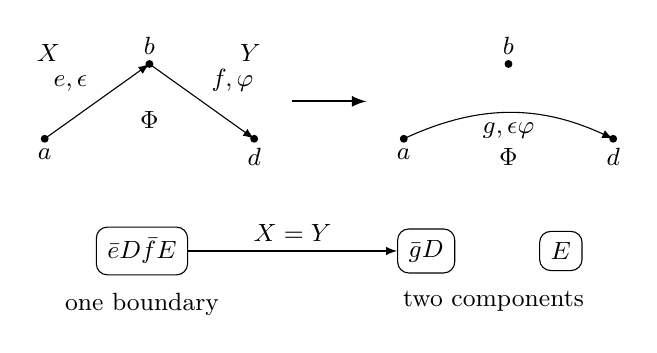
\begin{tikzpicture}[scale=.95,>=latex,every node/.style={font=\small}]
 \coordinate (a) at (-3.8,0);
 \coordinate (b) at (-2.4,1);
 \coordinate (d) at (-1,0);
 \draw[->] (a)--node[above left]{$e,\epsilon$}(b);
 \draw[->] (b)--node[above right]{$f,\varphi$}(d);
 \fill (a) circle (1.5pt) node[below]{$a$};
 \fill (b) circle (1.5pt) node[above]{$b$};
 \fill (d) circle (1.5pt) node[below]{$d$};
 \node at (-2.4,.25) {$\Phi$};
 \node at (-3.75,1.15) {$X$};
 \node at (-1.05,1.15) {$Y$};
 \draw[->,thick] (-.5,.5)--(.5,.5);
 \coordinate (aa) at (1,0);
 \coordinate (bb) at (2.4,1);
 \coordinate (dd) at (3.8,0);
 \draw[->] (aa) to[bend left=25] node[below]{$g,\epsilon\varphi$}(dd);
 \fill (aa) circle (1.5pt) node[below]{$a$};
 \fill (bb) circle (1.5pt) node[above]{$b$};
 \fill (dd) circle (1.5pt) node[below]{$d$};
 \node at (2.4,-.25) {$\Phi$};
 \node[draw,rounded corners,inner sep=4pt] (oldwalk) at (-2.5,-1.5)
   {$\bar eD\bar fE$};
 \node[draw,rounded corners,inner sep=4pt] (newwalk) at (1.3,-1.5)
   {$\bar gD$};
 \node[draw,rounded corners,inner sep=4pt] (otherwalk) at (3.1,-1.5)
   {$E$};
 \draw[->] (oldwalk)--node[above]{$X=Y$}(newwalk);
 \node[below=3pt] at (oldwalk.south) {one boundary};
 \node[below=3pt] at (2.2,-1.8) {two components};
\end{tikzpicture}
\caption{Smoothing two consecutive nonloop darts of one label.
All other incidences are omitted.  The opposite faces $X,Y$ may be
the same face; in that case its boundary splits as shown below the local
picture. The resulting drawing has two components, as the boundary-walk
calculation shows. If $E$ is empty, its component is the isolated vertex $b$.}
\label{fig:gluing-smoothing}
\end{figure}

Across the components, the total number of boundary walks increases
by one, the edge count decreases by one, and the vertex count is
unchanged.  Formula~\eqref{eq:gluing-euler} gives exactly two
components.  The new edge places $a,d$ in one of them.  Every component
must contain an endpoint of a removed edge, because the old graph was
connected; hence $b$ is in the other component.  In particular, the two
walks in~\eqref{eq:gluing-smooth-split} belong to different components.

Give both walks type $j$, and denote their evaluations by
\[
 A=(\epsilon\varphi)^{-1}D,\qquad B=E.
\]
The old word has evaluation $\epsilon^{-1}D\varphi^{-1}B$.
Moving the first factor $\epsilon^{-1}D$ to the end is a cyclic
change of starting point, so it preserves identity versus nonidentity.
The resulting evaluation is
\begin{equation}\label{eq:gluing-split-evaluation}
 (\varphi^{-1}B\varphi)A.
\end{equation}
If $X$ was exceptional, at least one of $A,B$ is nonidentity; retain
its component.  If $X$ was ordinary, $A$ and $B$ are either both
identity or both nonidentity.  In the former case keep the component
with the original exceptional face, whose evaluation is unchanged
even if it is $\Phi$.  In the latter keep the component without that
face; its new boundary is its sole exception.  This again gives a
smaller exceptional map.  We have proved that no face of the minimal
map has consecutive nonloop darts with equal labels, including the
last and first darts of its cyclic boundary walk.

\paragraph{Euler's formula rules out the minimal map.}
Consider a vertex that is not the base of a loop.  Reading the adjacent
face types around it gives a closed walk in $\Delta$.  Each incident
edge crosses between its two different endpoint types, and successive
edge labels are distinct by the smoothing reduction.  Thus the walk
has no immediate reversal.  Its length is positive since the connected
map has edges.  A simple triangle-free graph has no such closed walk
of length less than four, so this vertex has degree at least four.

An ordinary face not incident to a loop has a nonempty boundary walk.
Indeed every boundary walk of a connected graph with at least one
edge is a nonempty dart cycle; an empty walk occurs only for an isolated
vertex.  Its consecutive labels are distinct, and the short-word
condition~\eqref{eq:gluing-short-word} therefore forces its length to
be at least four.  Here and below a loop counts twice toward its
vertex degree, and boundary lengths count dart occurrences.

For our connected spherical map, Euler's formula and the two degree
sums give
\begin{equation}\label{eq:gluing-deficit}
 \sum_{v}(4-\deg v)+\sum_{F}(4-|\partial F|)=8.
\end{equation}
Without a loop, only the exceptional face can contribute positively,
and its nonempty walk contributes at most $3$.  With a loop, its base
vertex contributes at most $2$, the exceptional monogon contributes
$3$, and the face on the other side of the loop contributes at most
$2$: that face is ordinary and cannot have length one, since its sole
letter would be the loop's nonidentity value.  There are no other
loops, so every remaining vertex and face contributes at most zero.
The total is at most $2+3+2=7$, again contradicting
\eqref{eq:gluing-deficit}.  Consequently no exceptional map exists,
and every $D_i^0\to L$ is injective.

\paragraph{Extending to the full vertex groups.}
Let $\Omega=L\times\mathbb N$, with $L$ acting by left multiplication
on the first coordinate.  The restriction to each embedded $D_i^0$
is free and has countably infinitely many orbits.  The same is true
of the left $D_i^0$-action on $D_i\times\mathbb N$.  Pair their orbits
and choose one point in each pair; this determines a $D_i^0$-equivariant
bijection $D_i\times\mathbb N\to\Omega$.  Transport the free left
$D_i$-action along this bijection.  Its restriction to $D_i^0$ is
exactly the original $L$-action.  Make this choice separately for each
$i$.  The resulting actions agree on every edge group because both
copies of its chosen generator act as $x_\gamma\in L$.  They therefore
define an action of $Q$ on $\Omega$, faithful on every $D_i$.  This
proves the required injections.
\end{proof}

\subsection{Application to the modular construction}

Recall from Section~\ref{op:finite-section} the group
$H=A_0\rtimes P$, with $P=(\F_p)^3$ and
$A_0=(\mathbb Z/M\mathbb Z)^P$. Its subgroups
$U=u(P)$ and $V=cUc^{-1}$ satisfy $U\cap V=\{1\}$.
The quotient $G_0$ identifies, for every edge $i<j$, the elements
\begin{equation}\label{eq:gluing-embeddings}
 v(1,\bar j,\bar j^{2})\in H_i,
 \qquad u(1,\bar i,\bar i^{2})\in H_j,
\end{equation}
where $\bar i$ denotes the residue of $i$ in $\mathbb F_p$.
Both elements have order $p$, so the corresponding maps from $C_p$
are embeddings. We now verify the remaining local condition.

\begin{proposition}\label{prop:first-gluing-injective}
Every natural map $H_i\to G_0$ is injective.  In particular, the maps
$K[H_i]\to K[G_0]$ induced on group algebras are injective.
\end{proposition}

\begin{proof}
We verify the short-word hypothesis of
Lemma~\ref{lem:triangle-free-gluing}.  At a fixed vertex, every incident
edge subgroup lies either in $U$ or in $V$.  Within either subgroup,
the labels supplied by distinct neighbors $j$ correspond to the
vectors $(1,\bar j,\bar j^{2})$; a nonidentity syllable corresponds
to a nonzero scalar multiple of its vector.  Any three with distinct residues
are independent, because their determinant is, up to sign,
\[
 (\bar j_2-\bar j_1)(\bar j_3-\bar j_1)
 (\bar j_3-\bar j_2)\neq0.
\]
The residues are distinct since $p>m$.  The analogous first two
coordinates show independence for two vectors, and a single vector
is nonzero.  Thus a word of at most three nonidentity syllables with
distinct labels, all in $U$ or all in $V$, cannot evaluate to $1$.

For a mixed word of length two or three, one of $U,V$ supplies exactly
one syllable.  After a cyclic permutation, a putative relation would
equate that nonidentity syllable to a product of syllables from the
other subgroup. This contradicts $U\cap V=\{1\}$. For lengths
two and three, cyclically distinct consecutive labels are precisely
distinct labels, so all required words have been covered.  The graph
$\Gamma$ is simple and triangle-free, and all groups in question are
finite.  The lemma proves the injections.  The group-algebra assertion
follows because distinct elements of an embedded subgroup remain
distinct basis elements of $K[G_0]$.
\end{proof}
